\section[Jira : L'outil essentiel pour la gestion de projets]{Jira : L'outil essentiel pour la gestion quotidienne de projets}\label{sec:jira}

Au sein de l'entreprise, les équipes SCRUM se servent de Jira afin de consigner et de suivre tous les aspects de leur travail.

Jira est un outil essentiel pour les équipes SCRUM car il facilite la gestion complète du processus de développement agile. Il permet aux équipes de collaborer de manière efficace et de suivre chaque étape du cycle de vie du projet. Avec Jira, les équipes SCRUM peuvent créer, organiser et hiérarchiser leur Carnet de Produit en ajoutant des Histoires Utilisateurs, des tâches, des Épics et des bugs.

L'outil facilite la planification des sprints en permettant aux équipes de sélectionner les éléments du Carnet de Produit à inclure dans chaque itération. Les équipes peuvent estimer la complexité des tâches à l'aide de Story Points et suivre leur progression au fil du temps.

Les fonctionnalités de suivi des tâches et des problèmes dans Jira aident les équipes à gérer leur travail quotidien. Chaque membre de l'équipe peut mettre à jour l'état de ses tâches, signaler les obstacles et collaborer de manière transparente avec les autres membres de l'équipe.

Les réunions SCRUM telles que la Mêlée Quotidienne, la Revue de Sprint et la Rétrospective de Sprint peuvent être orchestrées efficacement grâce à Jira. L'outil permet de suivre les progrès, de partager les résultats et de documenter les réflexions pour chaque itération.

Les flux de travail (workflows) dans Jira constituent un mécanisme central pour orchestrer et suivre le déroulement des tâches et des projets. Ces flux définissent les étapes spécifiques à suivre pour qu'une tâche ou un problème progresse, de sa création à son achèvement. Les équipes peuvent personnaliser ces flux pour refléter leurs processus uniques, en définissant les transitions entre les étapes et en assignant des responsabilités à différents membres de l'équipe. Les flux de travail de Jira contribuent à maintenir la transparence, à améliorer l'efficacité et à garantir que toutes les parties prenantes restent informées de l'avancement du travail. Grâce à cette fonctionnalité, les équipes peuvent gérer avec agilité et précision les tâches, tout en favorisant une collaboration fluide et une visibilité accrue sur les projets.

Chez SuiviDeFlotte, le diagramme d'activité présenté dans la Figure~\ref{fig:lifecycle-of-incoming-ideas} est la base du flux de travail dans Jira. La partie supérieure gauche du diagramme illustre à nouveau le traitement des idées novatrices par les différents comités. En revanche, la partie supérieure droite présente le traitement des bogues (demandes courantes) qui proviennent de l'équipe de support. Ensuite, le propriétaire du produit sélectionne les tickets pour le prochain sprint à partir de l'ensemble des tickets prêts. Ce diagramme contient les étapes suivantes, qui sont utilisées comme étapes du flux de travail dans Jira : en raffinement, à faire, en cours, en test, à déployer, terminé, abandonné.

Un autre diagramme d'activité montre plus en détail le traitement des bogues (Figure~\ref{fig:lifecycle-of-bugs}). À partir de ce diagramme, nous pouvons ajouter quelques étapes supplémentaires à la liste des étapes du flux de travail : en attente, en attente support.

\begin{figure}[h]
    \centering
    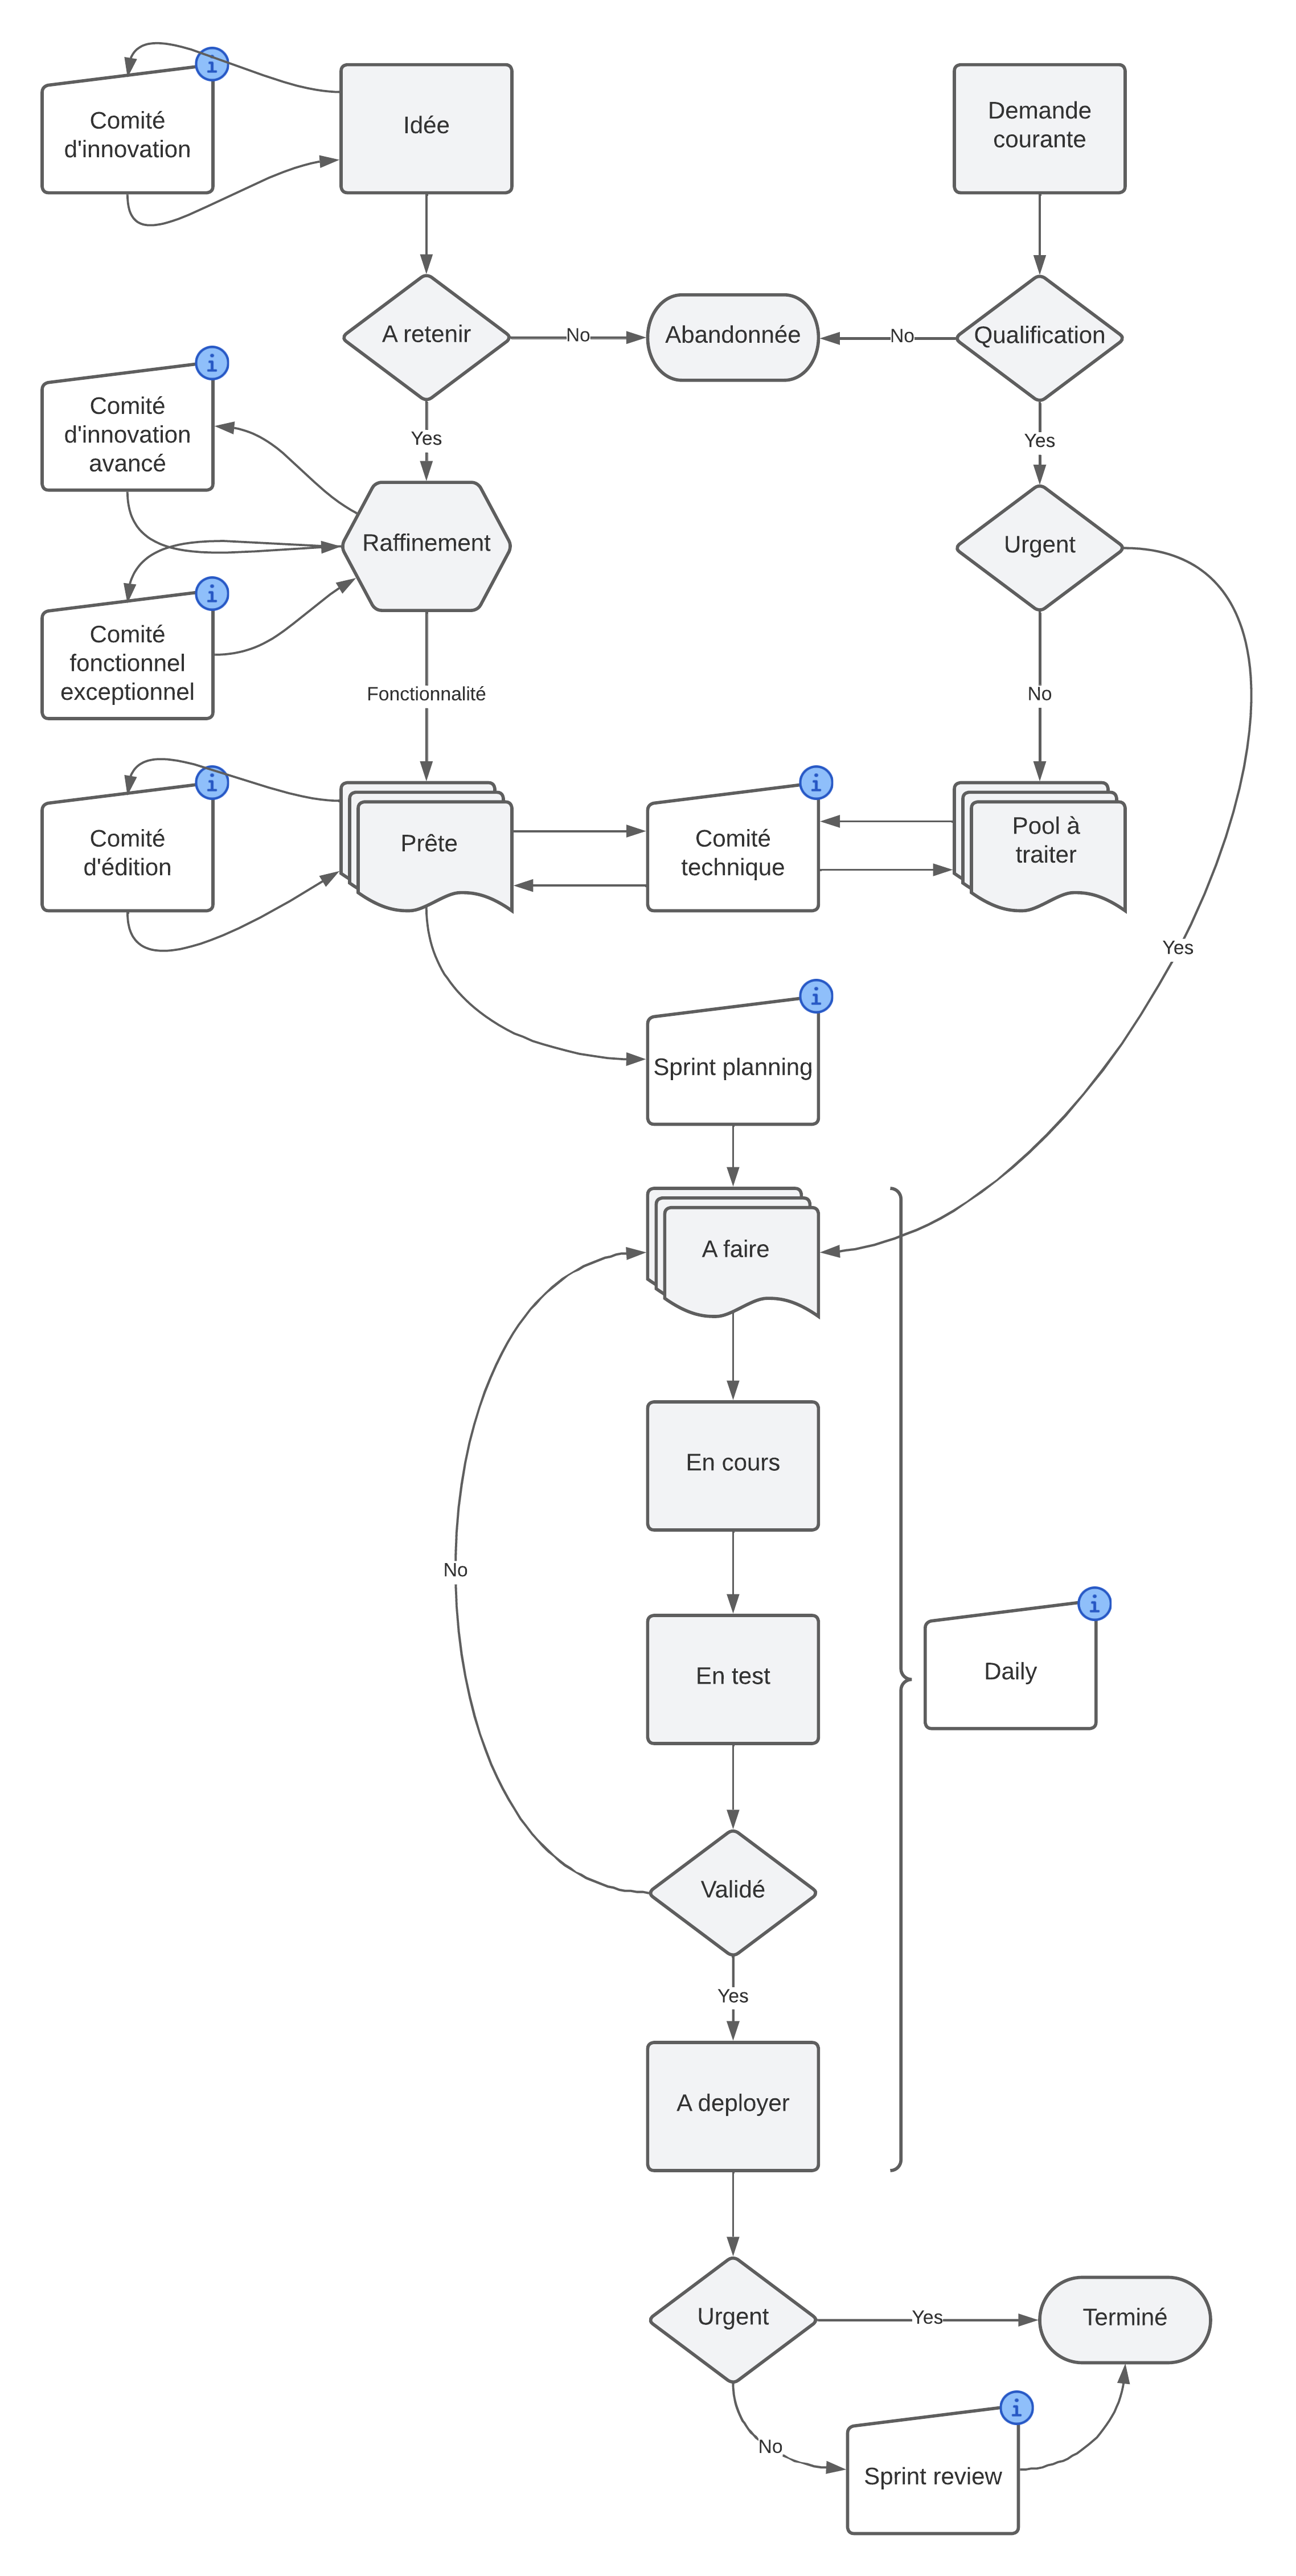
\includegraphics[height=0.9\textheight]{img/lifecycle-of-incoming-ideas}
    \caption{Diagramme d'activité du traitement des idées et des bogues (demandes courantes) entrants chez SuiviDeFlotte.}
    \label{fig:lifecycle-of-incoming-ideas}
\end{figure}

\begin{figure}[h]
    \centering
    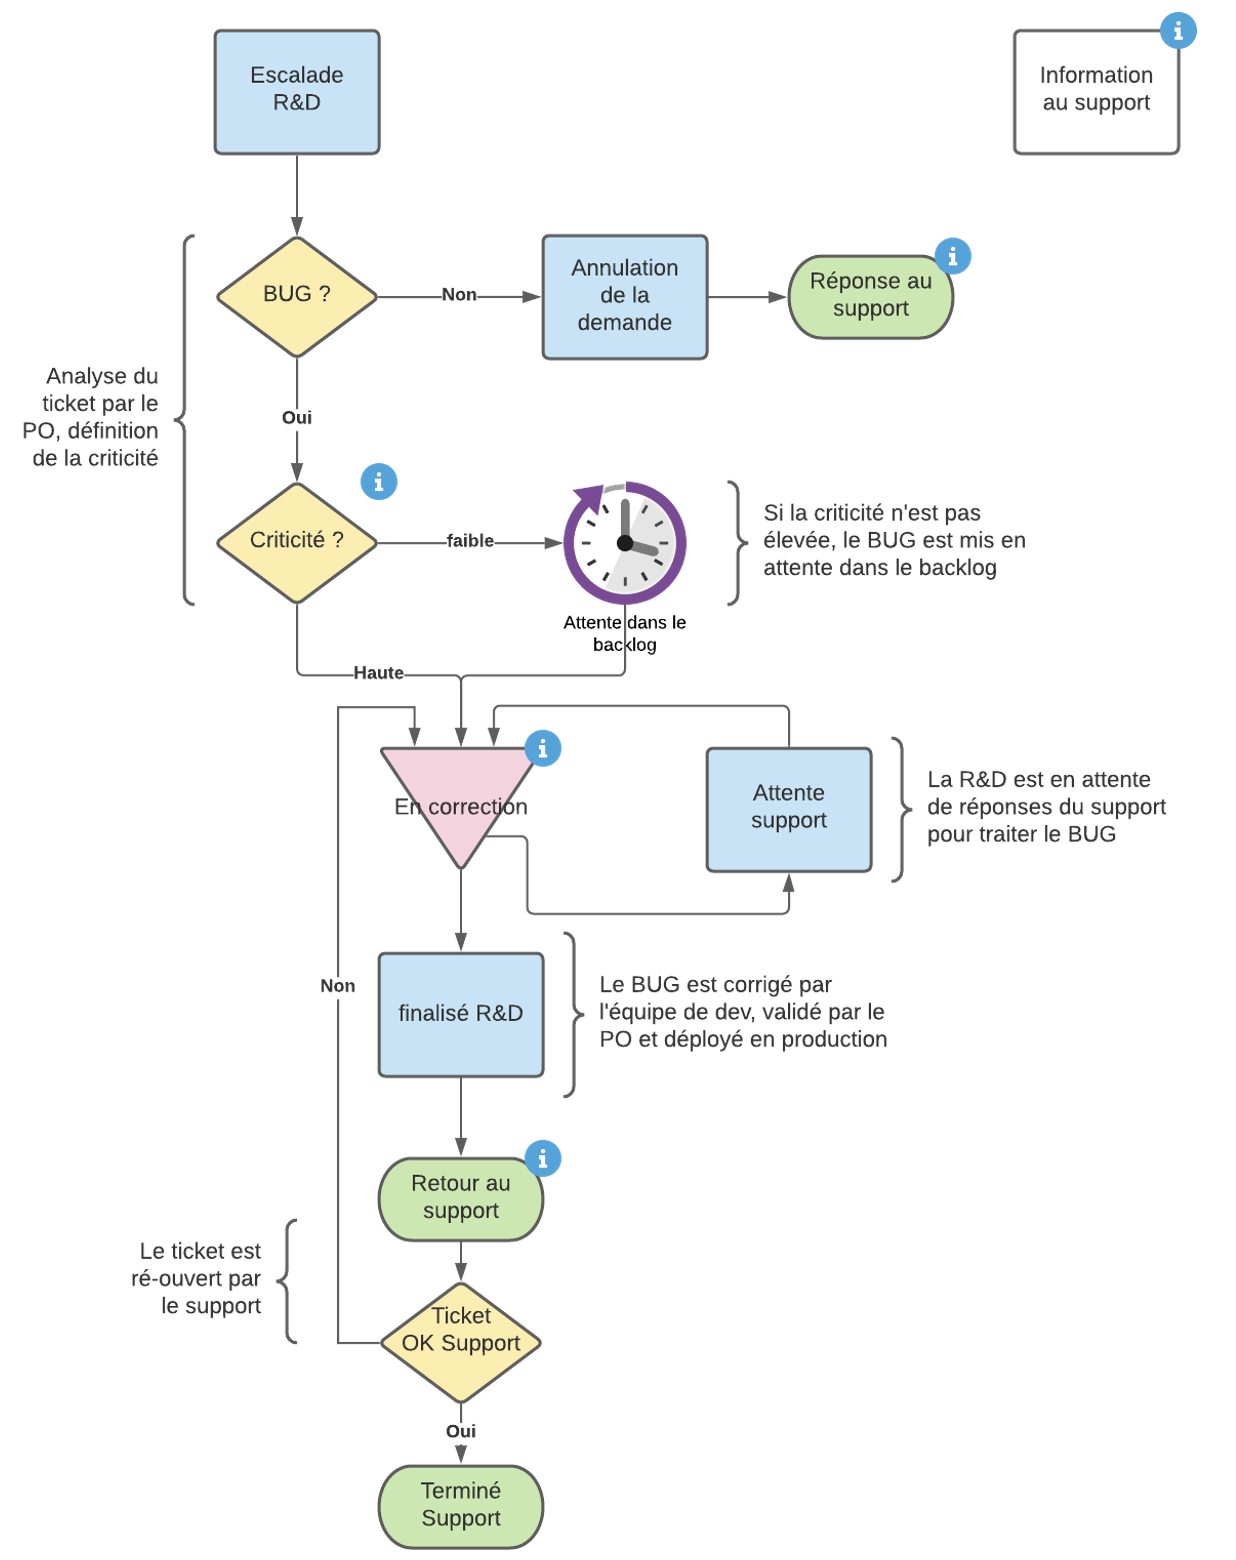
\includegraphics[width=\textwidth]{img/lifecycle-of-bugs}
    \caption{Diagramme d'activité du traitement des bogues.}
    \label{fig:lifecycle-of-bugs}
\end{figure}

Le diagramme de flux de travail qui en résulte et qui est actuellement utilisé est présenté à la Figure~\ref{fig:workflow}.

\begin{figure}[h]
    \centering
    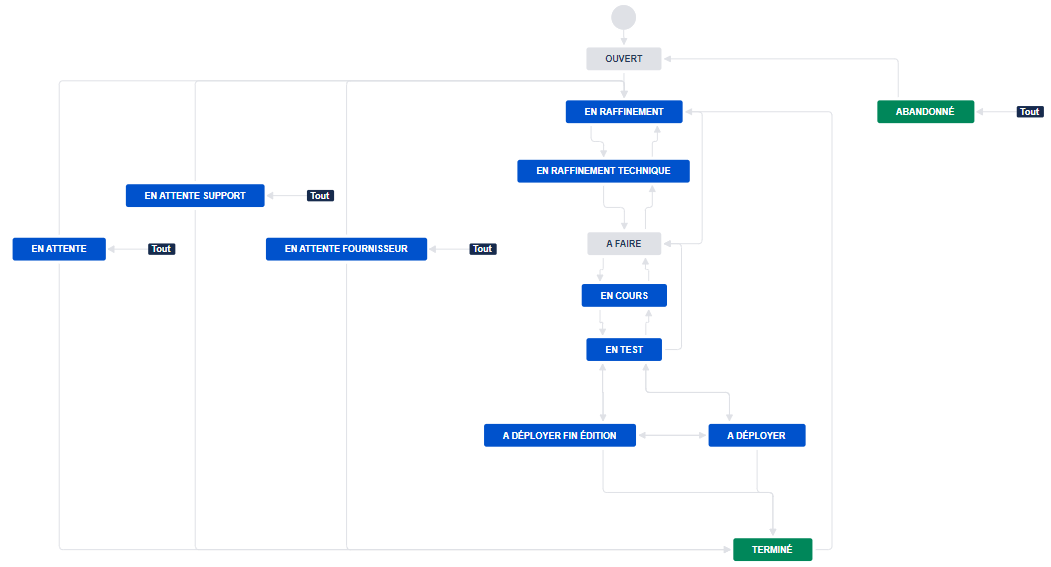
\includegraphics[width=\textwidth]{img/workflow-sdfn}
    \caption{Le flux de travail utilisé dans Jira chez SuiviDeFlotte.}
    \label{fig:workflow}
\end{figure}

La Figure~\ref{fig:product-backlog} et la Figure~\ref{fig:sprint} présentent un exemple de Backlog de produit et de Backlog de sprint sous forme de tableau Kanban, et la Figure~\ref{fig:ticket} donne un exemple d'un ticket.

\begin{figure}[h]
    \centering
    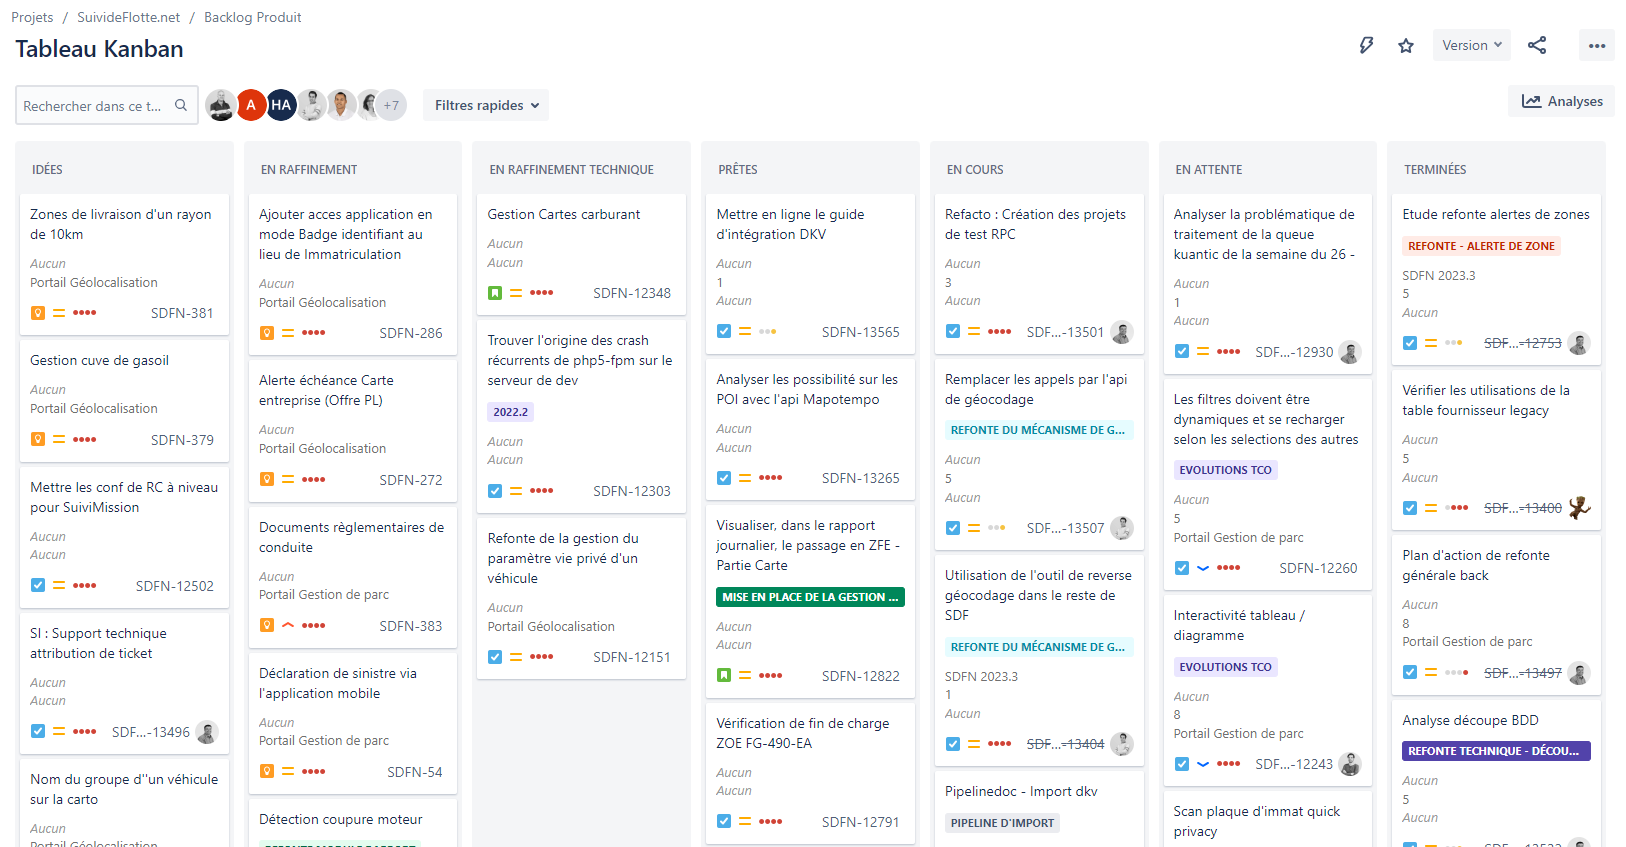
\includegraphics[width=\textwidth]{img/product-backlog}
    \caption{Le Backlog de produit sous forme de tableau Kanban dans Jira.}
    \label{fig:product-backlog}
\end{figure}

\begin{figure}[h]
    \centering
    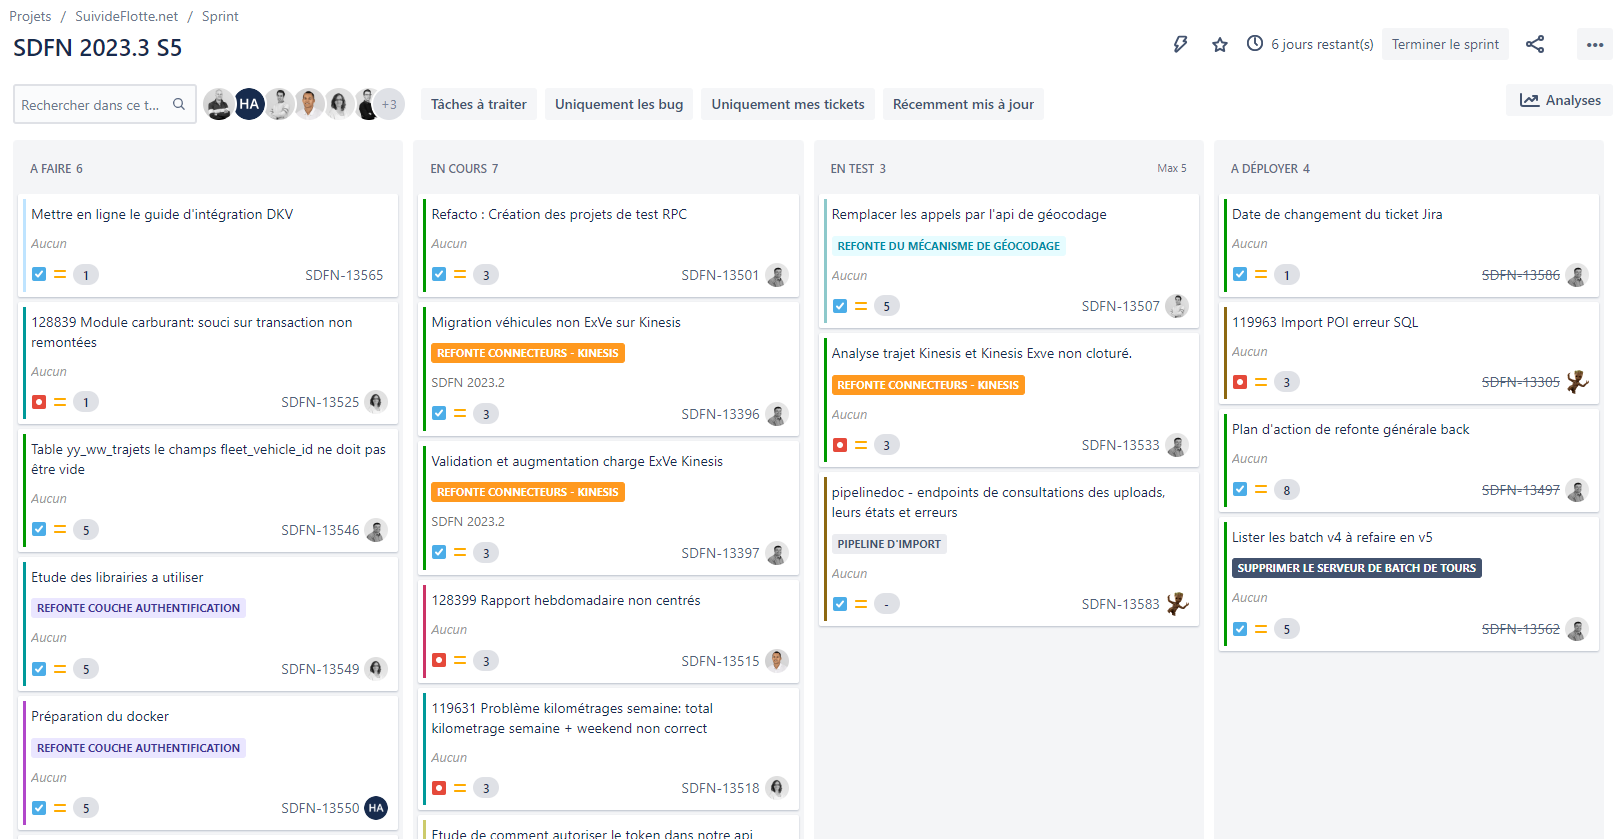
\includegraphics[width=\textwidth]{img/sprint}
    \caption{Le Backlog de sprint sous forme de tableau Kanban dans Jira.}
    \label{fig:sprint}
\end{figure}

\begin{figure}[h]
    \centering
    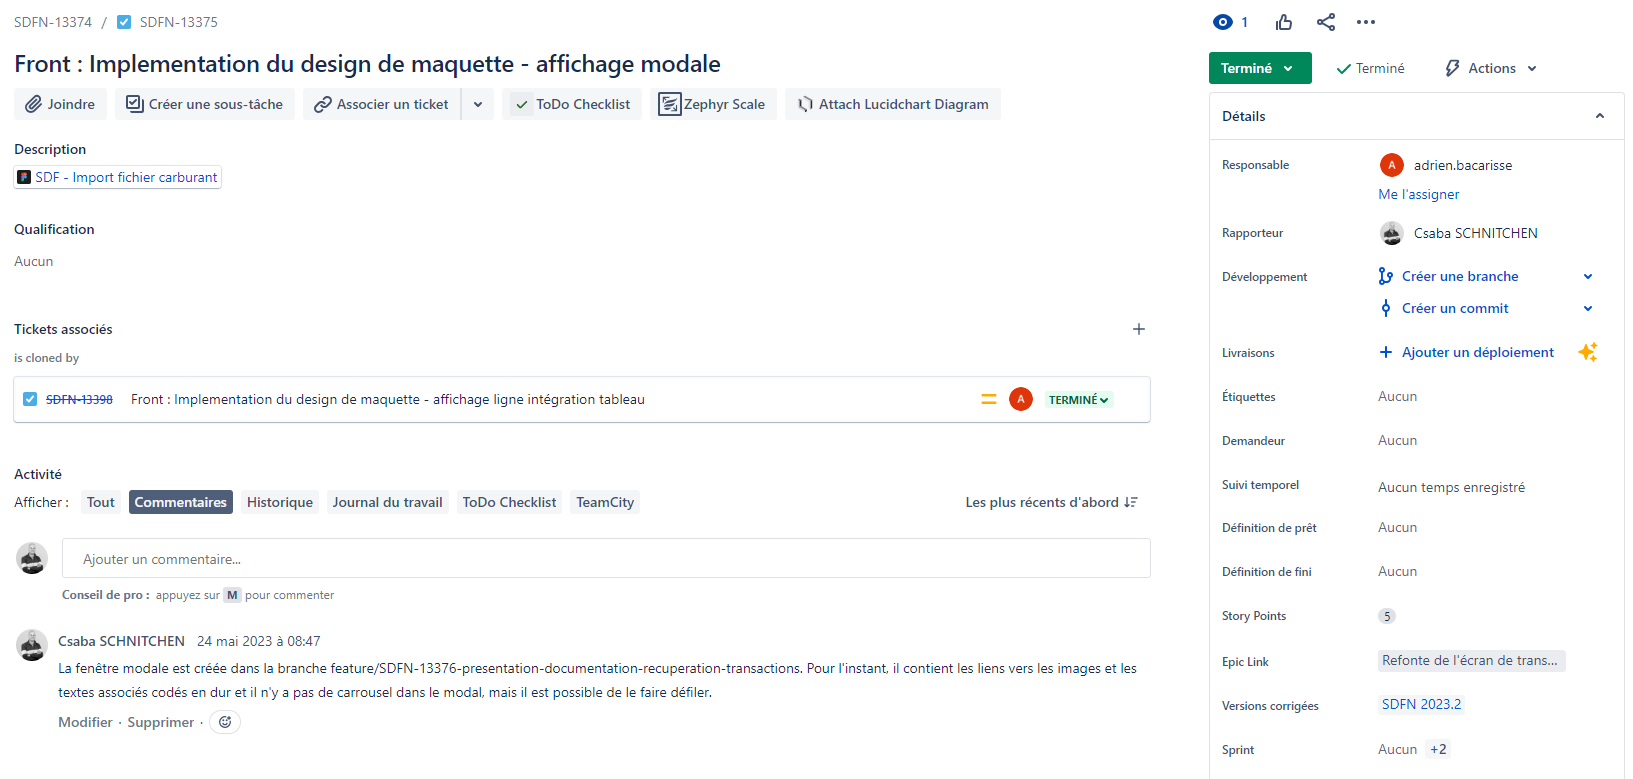
\includegraphics[width=\textwidth]{img/ticket}
    \caption{Un exemple de ticket dans Jira pour le projet d'amélioration de la page d'importation des fichiers des transactions de carburant.}
    \label{fig:ticket}
\end{figure}